\documentclass{beamer}

\usepackage{subcaption}
\usepackage[backend=bibtex]{biblatex}
\usepackage{media9}
\addbibresource{bib/main.bib}

\newcommand\fixme[2][FIXME]{\textcolor{red}{\textbf{#1:} #2}}
\usepackage[labelsep=space]{caption}
\usepackage[ruled, vlined, linesnumbered]{algorithm2e}

\SetKwInput{KwInput}{Input}
\SetKwInput{KwOutput}{Output}

\usepackage{amsmath}
\DeclareMathOperator*{\argmax}{arg\,max}

\usetheme[subsectionpage=progressbar, progressbar=frametitle]{metropolis}
\setbeamerfont{footnote}{size=\tiny}

\definecolor{turquoise}{RGB}{64,224,208}
\definecolor{turqbrown}{RGB}{92,80,60}
\setbeamercolor{progress bar}{fg=turquoise}
\setbeamercolor{normal text}{fg=turqbrown}
\title{Safe and Efficient Robotic Control via Piecewise-Affine Reinforcement Learning}
\author{\textbf{W. Cannon Lewis II}, Marzia Cescon, Lydia Kavraki}

\date{February 21, 2022}

\begin{document}
\begin{frame}
  \titlepage
\end{frame}

\section{Motivation}

\begin{frame}{Industrial Robotics}
  Industrial robots are heavy, dangerous, and expensive

  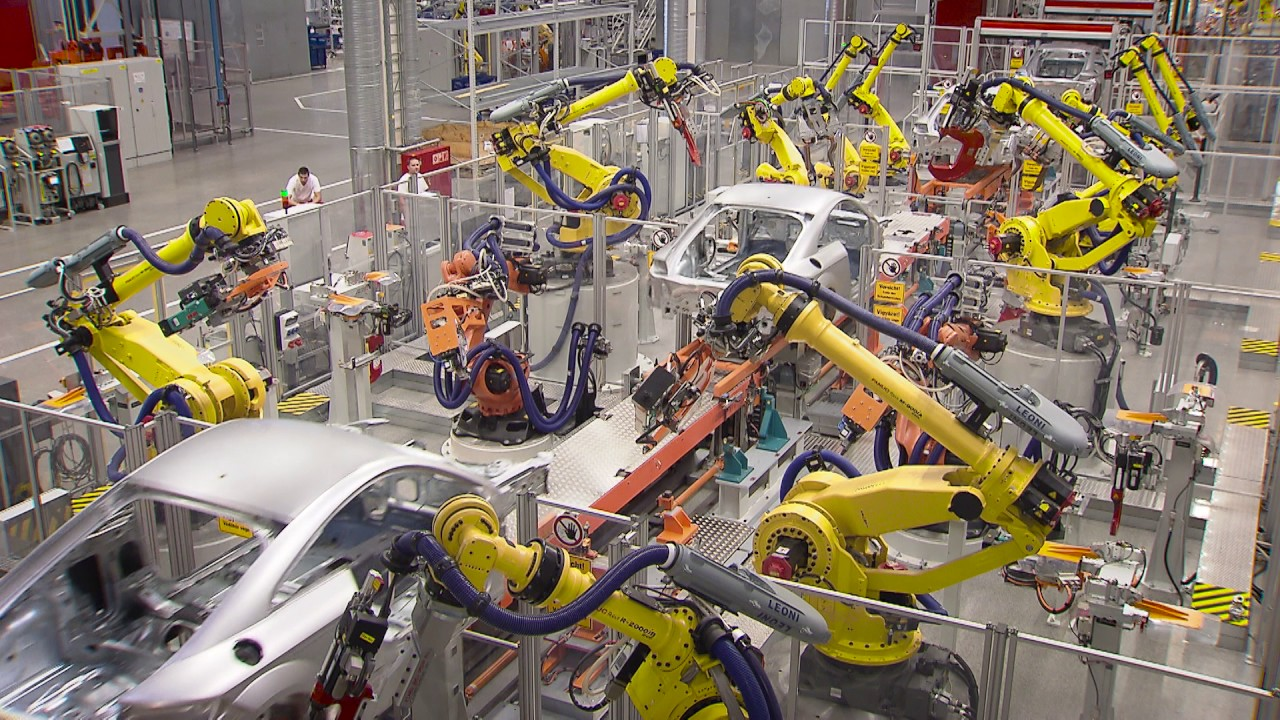
\includegraphics[keepaspectratio,width=\textwidth]{assets/factory_robots}
\end{frame}

\begin{frame}{Beyond Industrial Robots}
  Agile robots like Spot are still expensive and require extensive human guidance.

  \begin{center}
    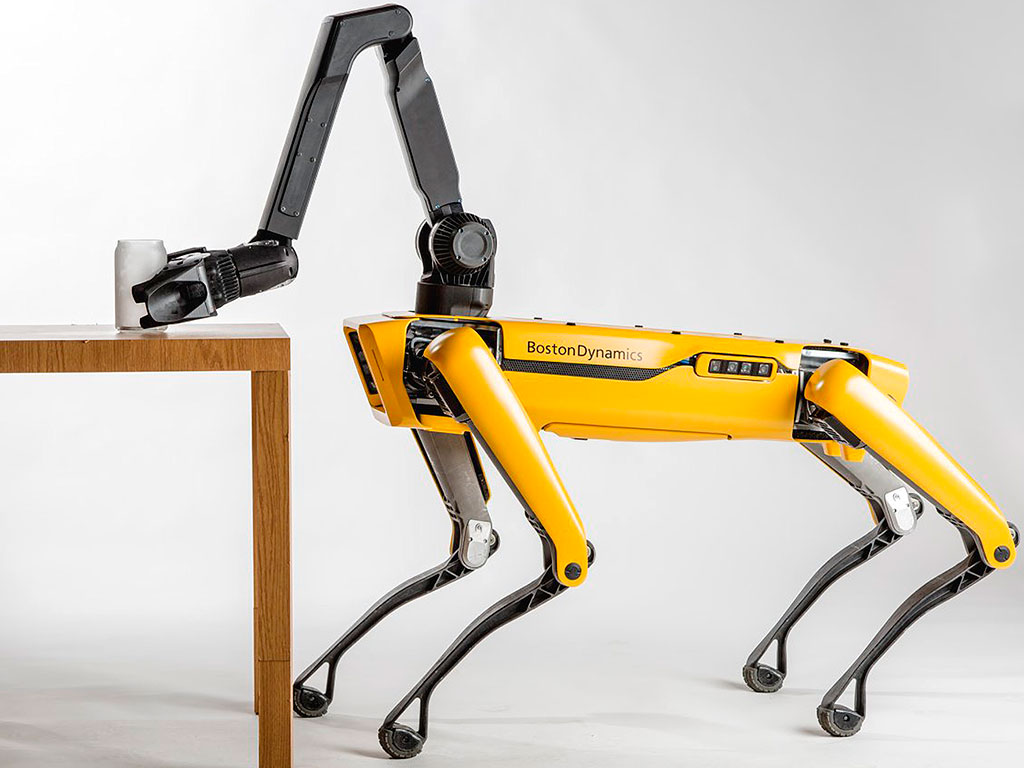
\includegraphics[keepaspectratio,width=0.8\textwidth]{assets/spotmini}
  \end{center}
\end{frame}

\begin{frame}{Learning to the Rescue?}
  There has been a lot of interest in learning for robot control and motion
  planning recently.

  \begin{center}
    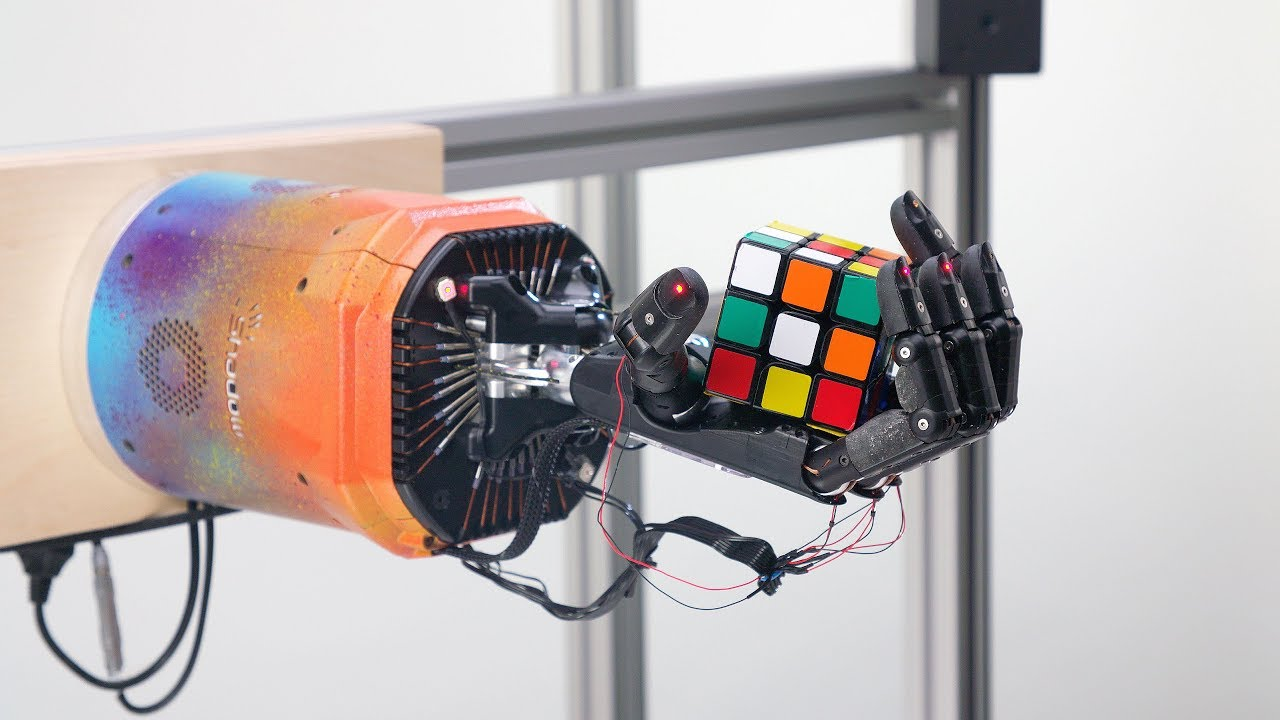
\includegraphics[keepaspectratio,width=\textwidth]{assets/openai_hand}
  \end{center}
\end{frame}

\begin{frame}{Big Data and Large Models}
  Deep learning leads us right back to expensive robots and questionable
  generalization. 

  Where is learning taking place?

  \begin{center}
    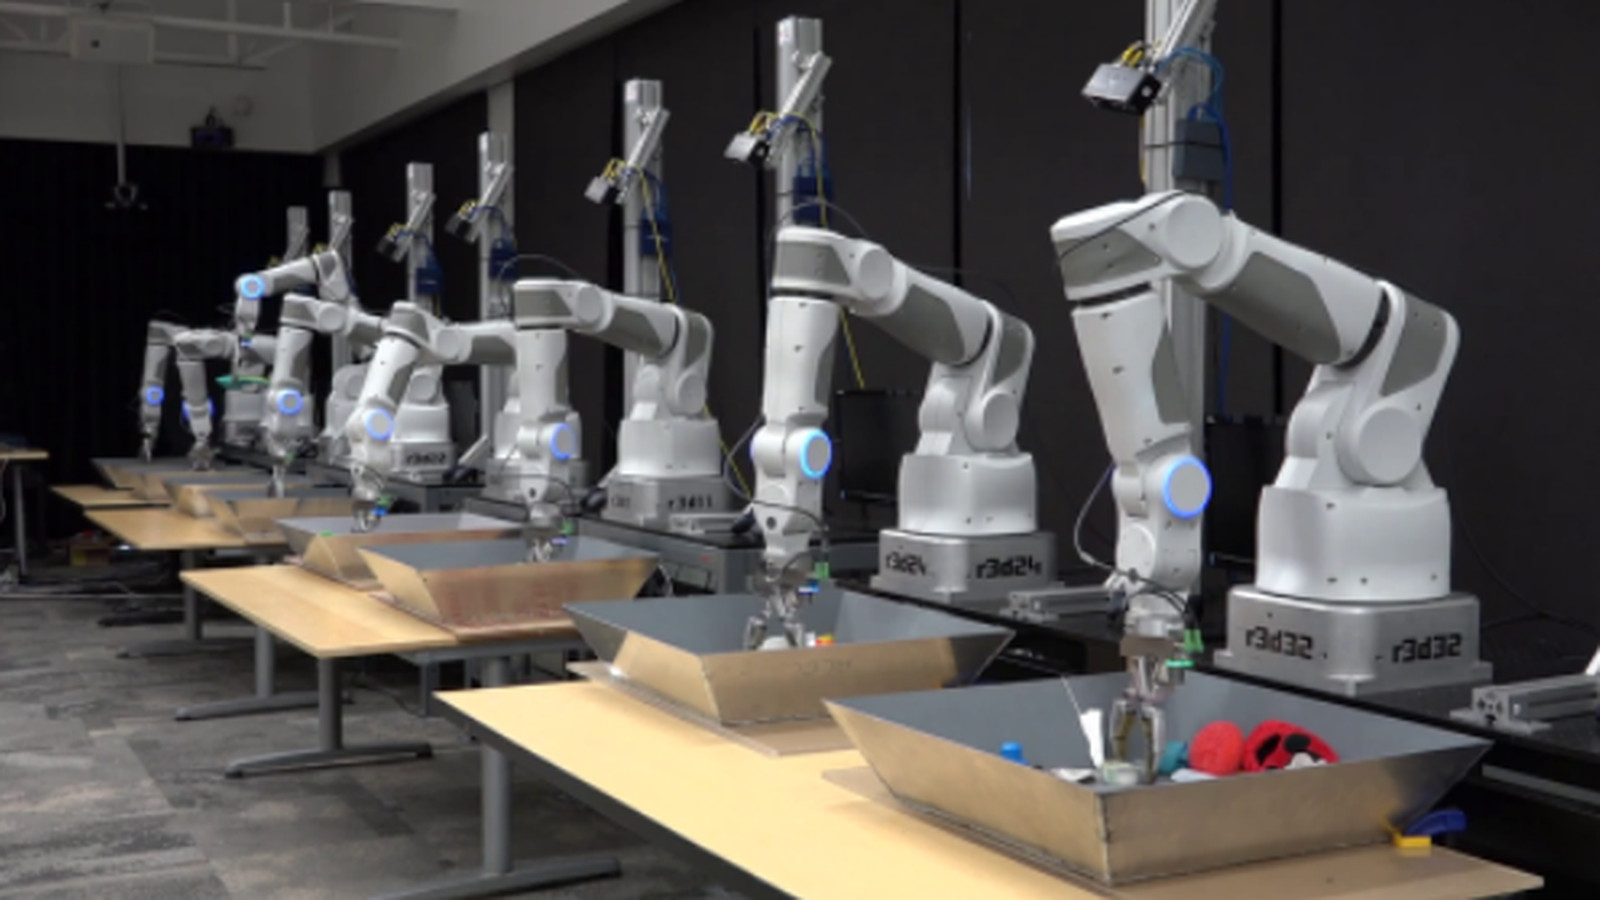
\includegraphics[keepaspectratio,width=0.8\textwidth]{assets/arm_farm}
  \end{center}
\end{frame}

\section{Reinforcement Learning}

\begin{frame}{RL Basics}
  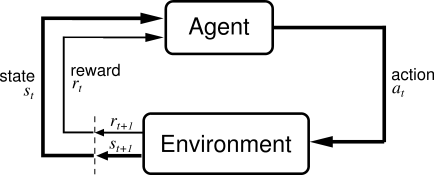
\includegraphics[keepaspectratio,width=\textwidth]{assets/agent_env}
\end{frame}

\begin{frame}{Notation}
  \begin{itemize}
    \item $x_t \in X$ (or $s_t$) are states, $u_t \in U$ (or $a_t$) are actions. 
    \item $r_t \in \mathbb{R}$ is a reward given by a \emph{reward function} $R : X \times U \rightarrow \mathbb{R}$.
    \item $P: X \times U \rightarrow X$ is a transition function.
    \item $\pi: X \rightarrow U$ is a \emph{policy} (or controller).
  \end{itemize}
\end{frame}

\begin{frame}{Value Functions}
  State value function\footfullcite{Sutton1998IntroductionTR}:
  \begin{equation}
    V_\pi(x) = \mathbb{E}\left[\sum_{t=0}^\top \gamma^t R(x_t, \pi(x_t)) \mid x_0 = x\right]
  \end{equation}
  satisfies Bellman equation
  \begin{equation}
    V_\pi(x) = \mathbb{E}\left[R(x, \pi(x)) + \gamma V_\pi(x_{t+1})\right]
  \end{equation}
\end{frame}


\section{PARL in Three Parts}
\begin{frame}{Piecewise-Affine Reinforcement Learning}
  \scalebox{0.7} {
  \begin{algorithm}[H]
    \DontPrintSemicolon
    \SetAlgoLined
    \SetKwInOut{Input}{Input}
    \SetKwInOut{Output}{Output}
    \Input{A system to be controlled}
    \Output{A learned PARL controller}

    Sample reference points within state-space of $env$. \\
    Initialize $\hat{F}, \hat{V}$, and $\Pi$ to sensible defaults. \\
    \For{$i$ = $1\ldots training\_iterations$} {
      $data \leftarrow \emptyset$ \\
      \For{$j$ = $1\ldots num\_rollouts$} {
        $traj = do\_rollout(\Pi, env)$ \\
        $register\_experience(traj)$ \\
        $update\_dynamics(\hat{F})$ \\
        $update\_value\_function(\hat{V})$ \\
        $data \leftarrow data \cup traj$ \\
      }
      $update\_controller(\Pi, data)$ \\
      $data \leftarrow \emptyset$ \\
    }
    Return $\Pi$
    \caption{PARL}
  \end{algorithm}
  }
\end{frame}

\subsection{Partitioning}

\begin{frame}{What is a Partition?}
  We can loosely define a partition with indexing set $I$ of the state space $X$ as
  \begin{equation}
    P_I = \left\{\mathcal{V}_i \subseteq S\ \middle\vert 
      \begin{array}{l}
        i \in I, \\
        \bigcup_{i \in I}\mathcal{V}_i = S, \\
        \mathcal{V}_i \cap \mathcal{V}_j = \emptyset, \forall i \neq j
      \end{array}\right\}
  \end{equation}
\end{frame}

\begin{frame}{Implicit Voronoi Partition}
  Explicit polygonal partitions are expensive, so we define an implicit one by
  sampling \emph{reference points} and using a K-D Tree to establish region membership.\footfullcite{de1997computational}

  \begin{center}
    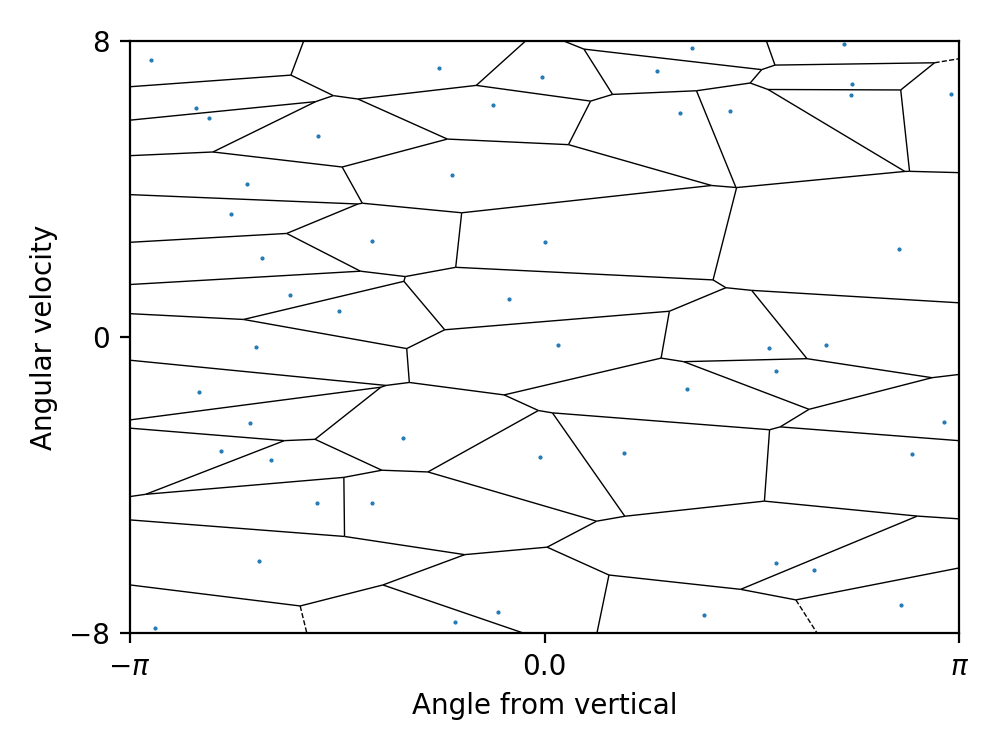
\includegraphics[keepaspectratio,width=0.7\textwidth]{assets/pendulum_voronoi}
  \end{center}
\end{frame}

\begin{frame}{Connections to Deep Neural Networks}
  Common deep neural network structures define implicit generalized Voronoi
  diagrams and piecewise-affine operators.\footfullcite{Balestriero2019TheGO} 

  \begin{center}
    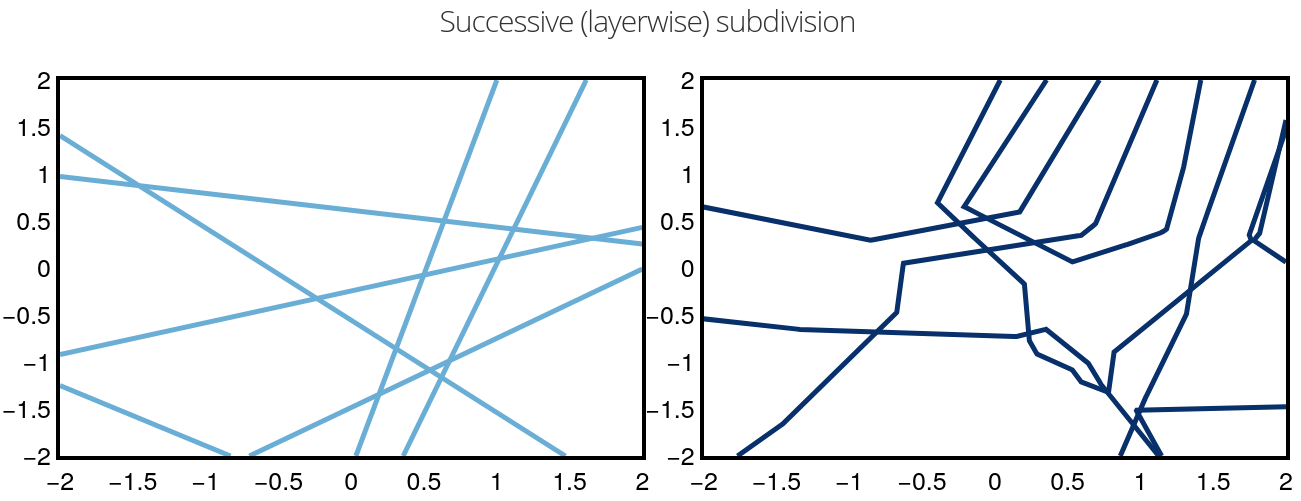
\includegraphics[keepaspectratio,width=0.8\textwidth]{assets/subdivision}
  \end{center}
\end{frame}

\subsection{Dynamics Estimation}

\begin{frame}{Local Linear Dynamics}
  We make a linear approximation to the local dynamics:
  \begin{equation}
    \hat{F}_{i}(\tilde{x}_t, u_t) = \hat{A}x_t + \hat{B}u_t + c 
  \end{equation}
  which can be estimated from data using \emph{Recursive Least Squares}
\end{frame}

\subsection{Value Function Approximation}

\begin{frame}{Local Value Function Approximation}
  Similar to the dynamics approximation, we make a linear approximation of the local dynamics:
  \begin{equation}
    \hat{V}^{\pi}_i(x_t) = V_0 + V_x^\top x_t
  \end{equation}
  which can be estimated using \emph{Least Squares Temporal Difference Learning}.
\end{frame}

\begin{frame}{Practical Implementation}
  For PARL, we define
  \begin{align*}
    \phi_i(x_t) &= \begin{cases} \begin{bmatrix} x_t \\ 1 \end{bmatrix} & \text{for } x \in \mathcal{V}_i \\ 0  &\text{otherwise}\end{cases} \\
    \phi_T(x_t) &= \phi_i(x_t) \text{, stacked for all $i \in I$}
  \end{align*}
  This feature set leads to a self-consistent piecewise-affine approximation to
  the value function on the PARL partition.
\end{frame}

\subsection{Controller Optimization}

\begin{frame}{Gradient-based Controller Updating}
    We optimize a piecewise-affine controller in terms of local linear controllers defined by
  \begin{equation}
    \pi_i(x_t) = Kx_t + k
  \end{equation}

  It is easy to compute empirical gradients of $V$ with respect to the local
  controller parameters $K$ and $k$ that apply at a state $x_t$:
  \begin{align}
    \nabla_K &= B^\top V_x x_t^\top \\
    \nabla_k &= B^\top V_x
  \end{align}
  Since we have a full estimate of the dynamics and value function, we can also
  do a line search rather than using a learning rate parameter. 
\end{frame}

\subsection{Results}

\begin{frame}{The Inverted Pendulum}
  \begin{figure}
    \centering
    \begin{subfigure}{0.8\linewidth}
      \centering
      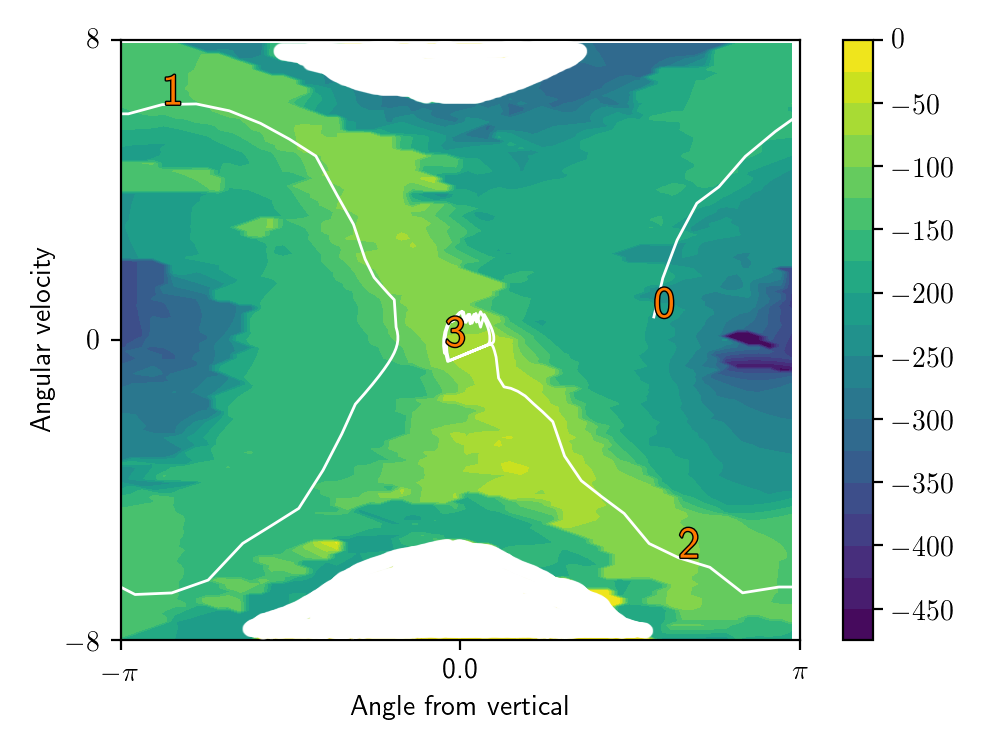
\includegraphics[width=\linewidth,trim=0 10 0 0,clip]{assets/pendulum_value}
      \vspace{-1em}
    \end{subfigure}
    \begin{subfigure}{0.2\linewidth}
      \centering
      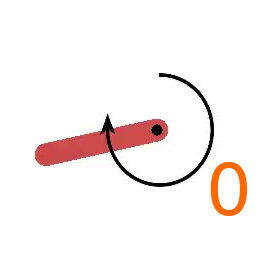
\includegraphics[width=\linewidth,trim=0 0 0 20]{assets/pendulum_traj_0}
    \end{subfigure}
    \begin{subfigure}{0.2\linewidth}
      \centering
      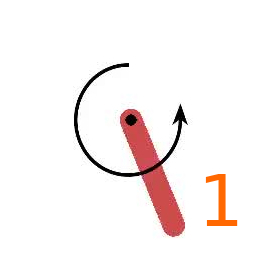
\includegraphics[width=\linewidth,trim=0 0 0 20]{assets/pendulum_traj_1}
    \end{subfigure}
    \begin{subfigure}{0.2\linewidth}
      \centering
      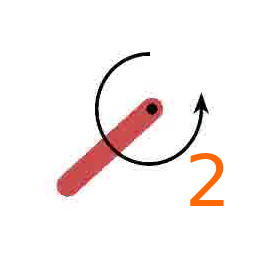
\includegraphics[width=\linewidth,trim=0 0 0 20]{assets/pendulum_traj_2}
    \end{subfigure}
    \begin{subfigure}{0.2\linewidth}
      \centering
      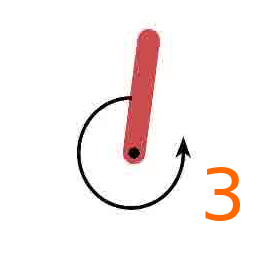
\includegraphics[width=\linewidth,trim=0 0 0 20]{assets/pendulum_traj_3}
    \end{subfigure}
  \end{figure}
\end{frame}

\begin{frame}{Reference Point Placement Experiments}
  \begin{figure}[htb]
      \centering
      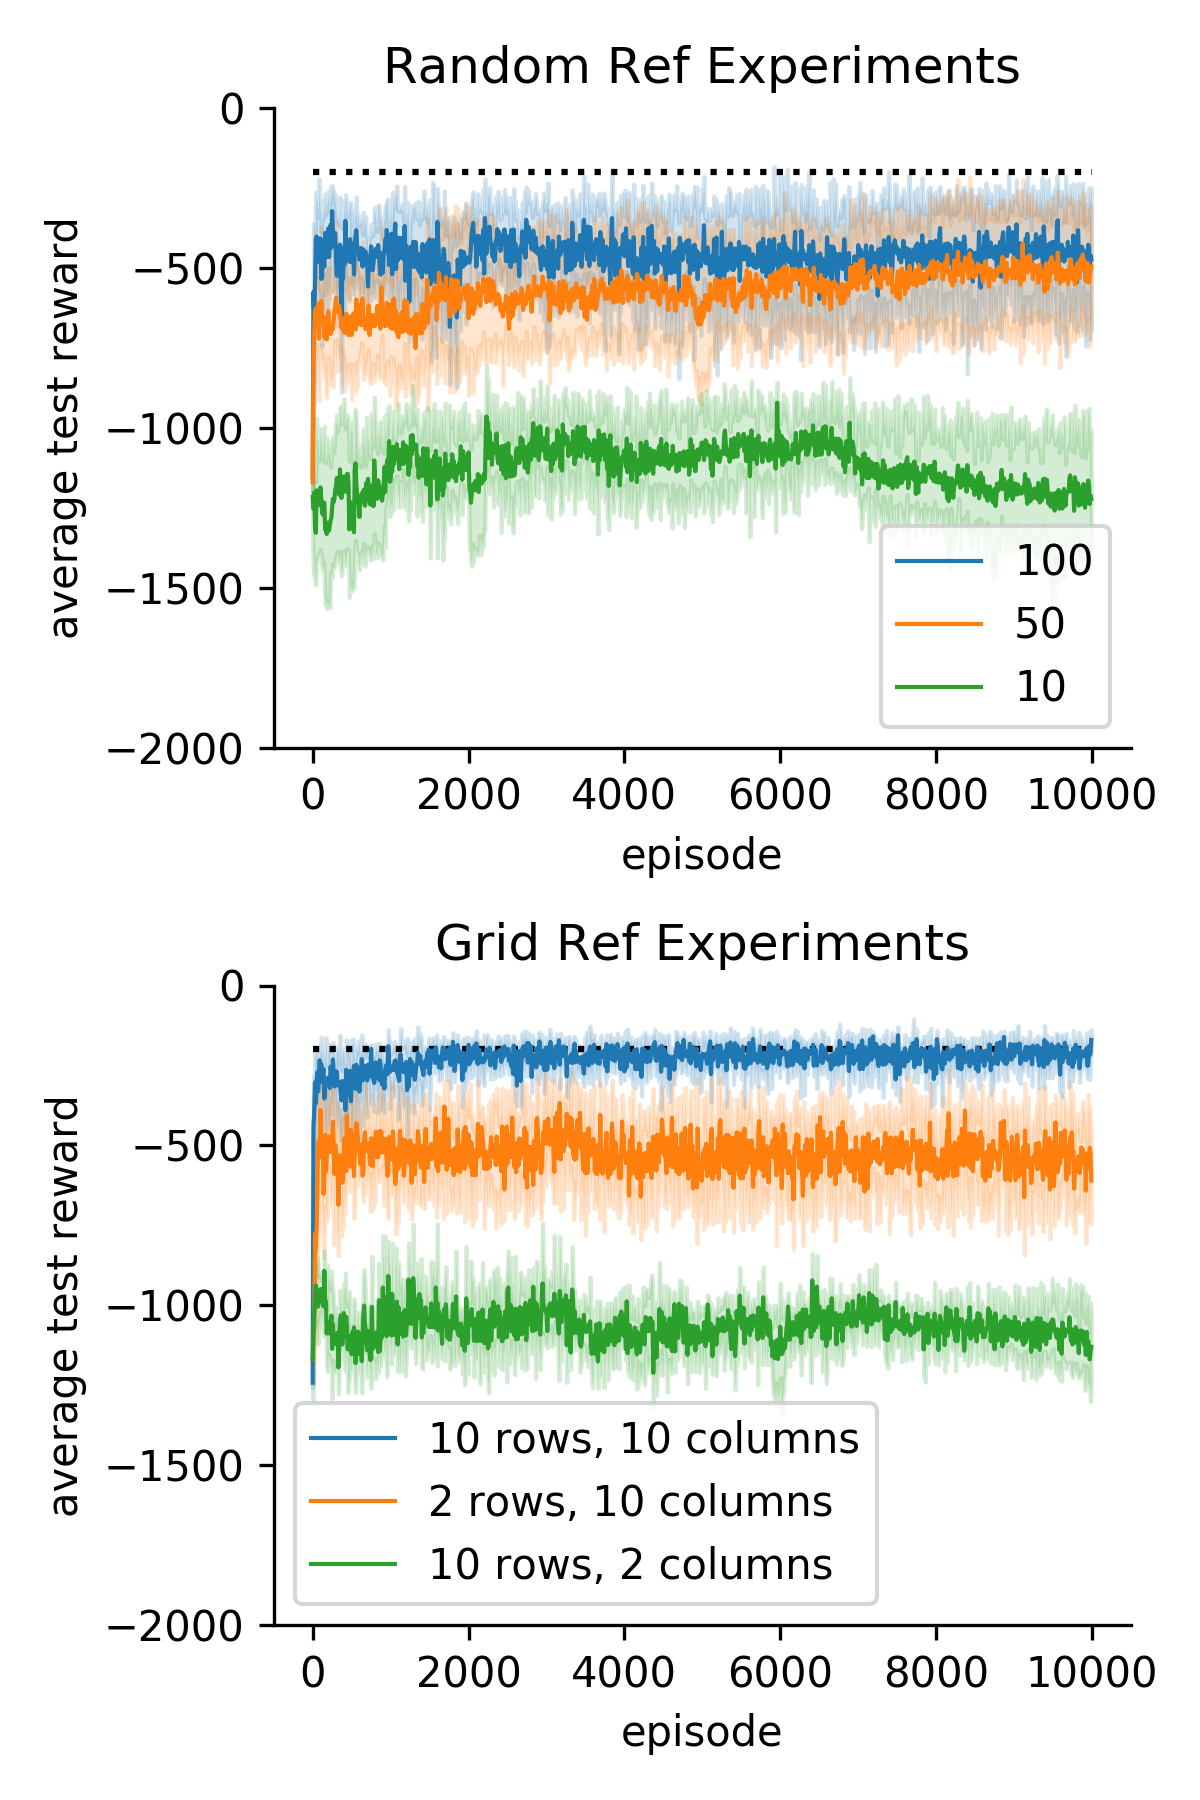
\includegraphics[width=0.5\linewidth,trim=0 0 0 0,clip]{assets/combined_ref_exps}
  \end{figure}
\end{frame}

\begin{frame}{Interpretability Experiments: Value Functions}
  \begin{figure}[t]
    \centering
    \begin{subfigure}{0.30\linewidth}
      \centering
      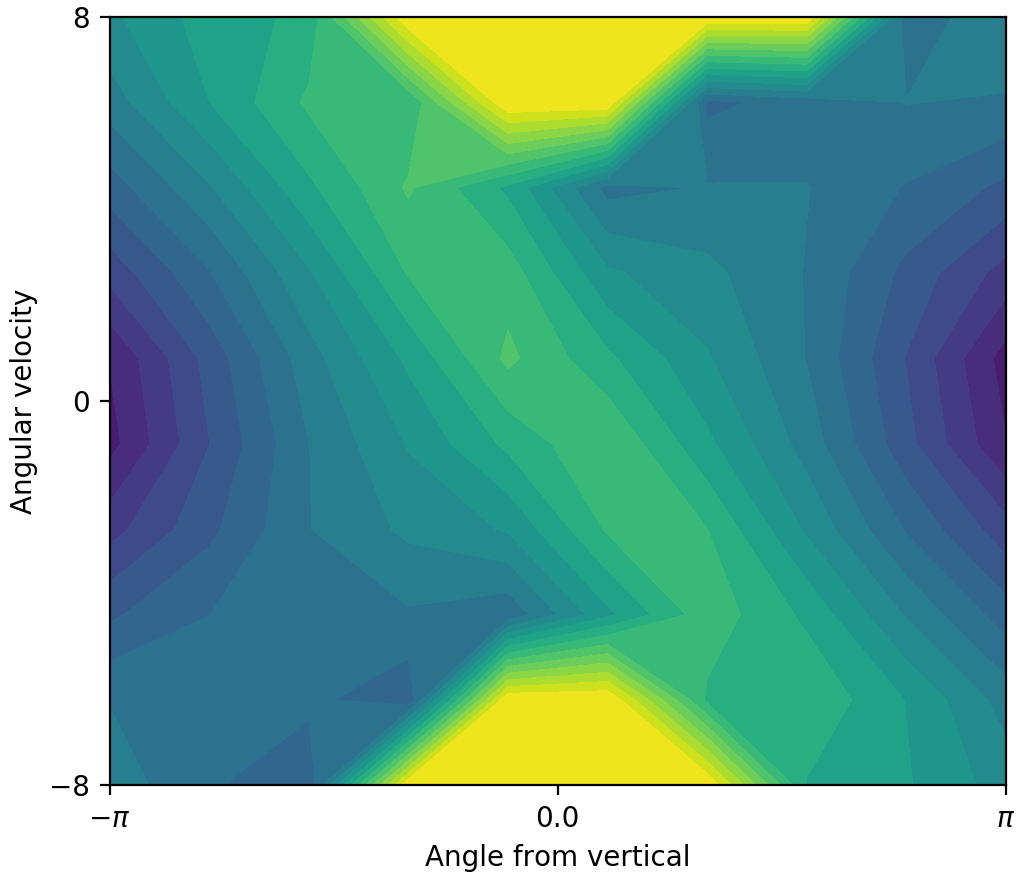
\includegraphics[width=0.9\linewidth,trim=0 0 0 0,clip]{assets/ref_plots/value_model_refcolexps_r10c10_1_ep0}
      \caption{0 episodes}
    \end{subfigure}
    \begin{subfigure}{0.30\linewidth}
      \centering
      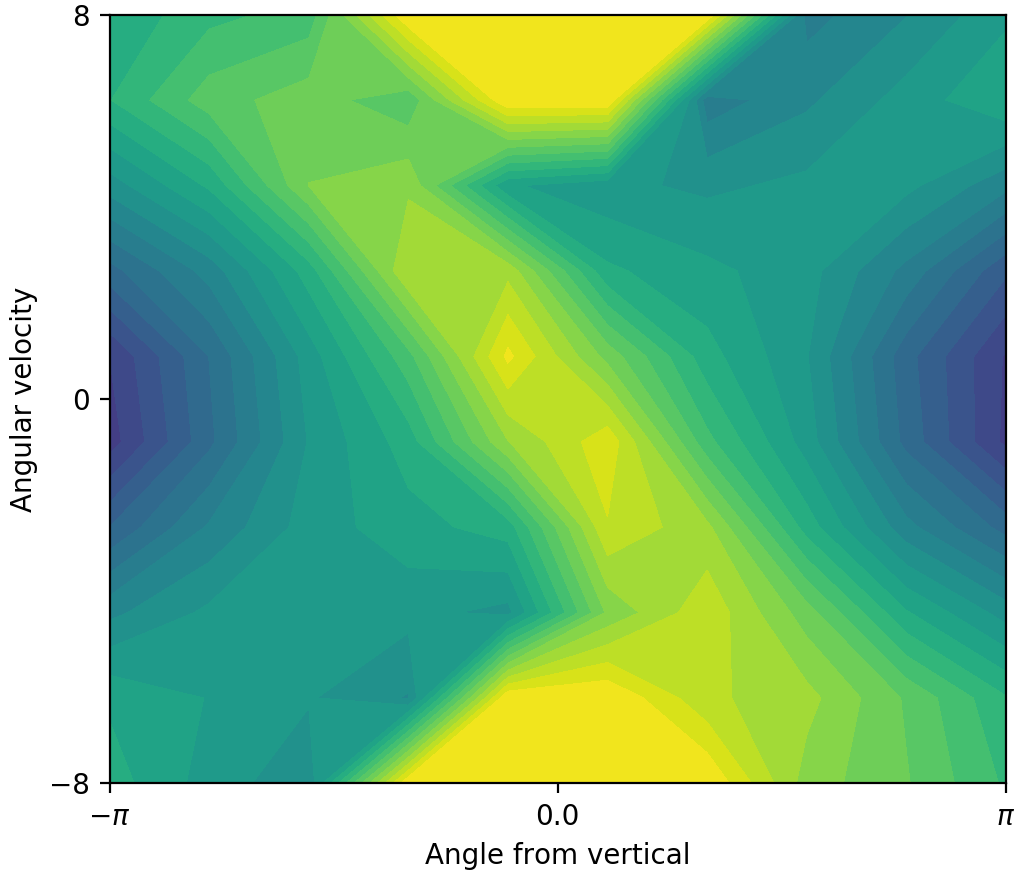
\includegraphics[width=0.9\linewidth,trim=0 0 0 0,clip]{assets/ref_plots/value_model_refcolexps_r10c10_1_ep1000}
      \caption{1000 episodes}
    \end{subfigure}
    \begin{subfigure}{0.30\linewidth}
      \centering
      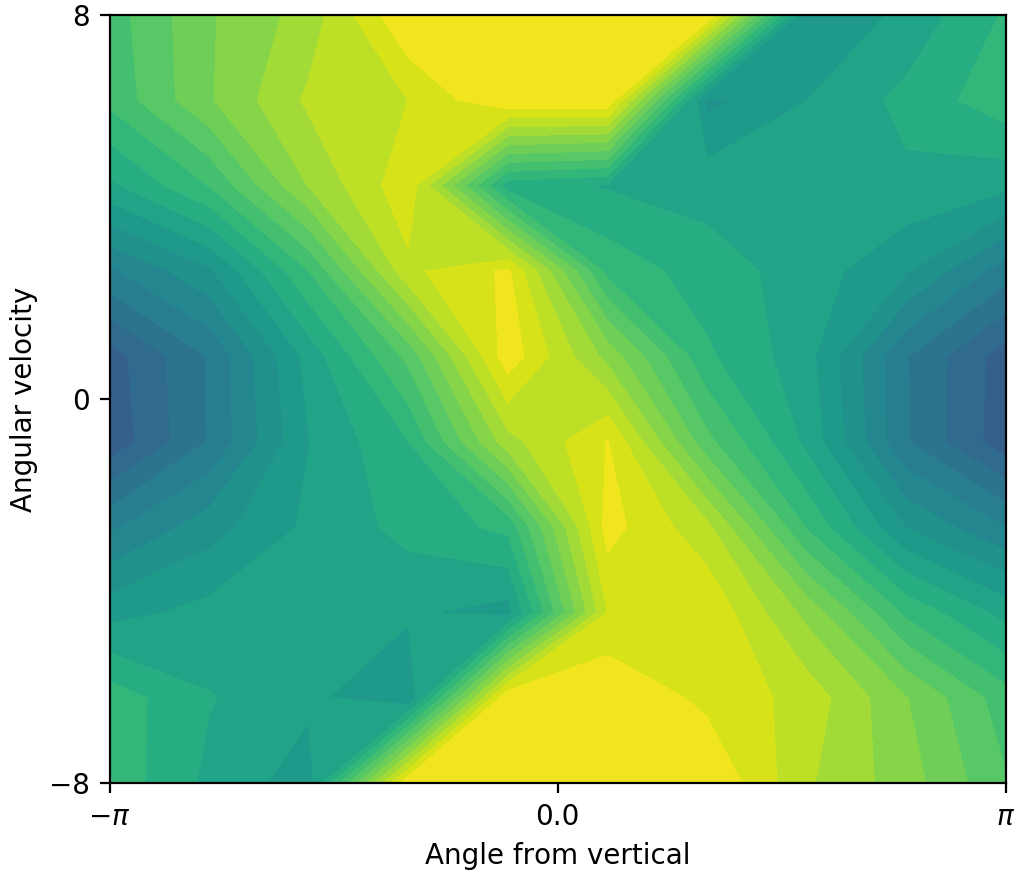
\includegraphics[width=0.9\linewidth,trim=0 0 0 0,clip]{assets/ref_plots/value_model_refcolexps_r10c10_1_ep9900}
      \caption{9900 episodes}
    \end{subfigure}
    \begin{subfigure}{0.05\linewidth}
      \vspace{-2em}
      \centering
      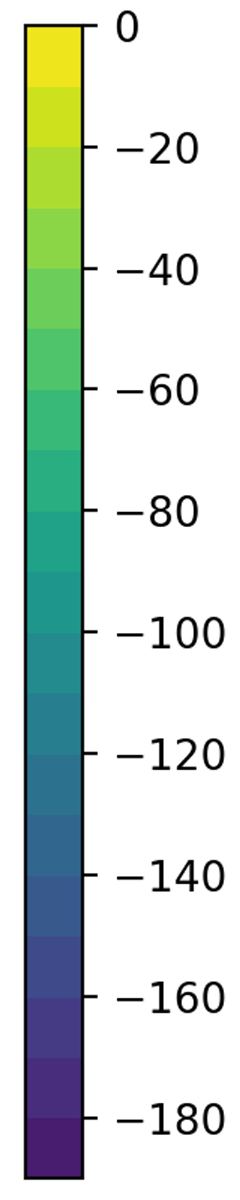
\includegraphics[width=\linewidth,trim=0 0 0 0,clip]{assets/ref_plots/r10c10_colorbar}
    \end{subfigure}
    \begin{subfigure}{0.30\linewidth}
      \centering
      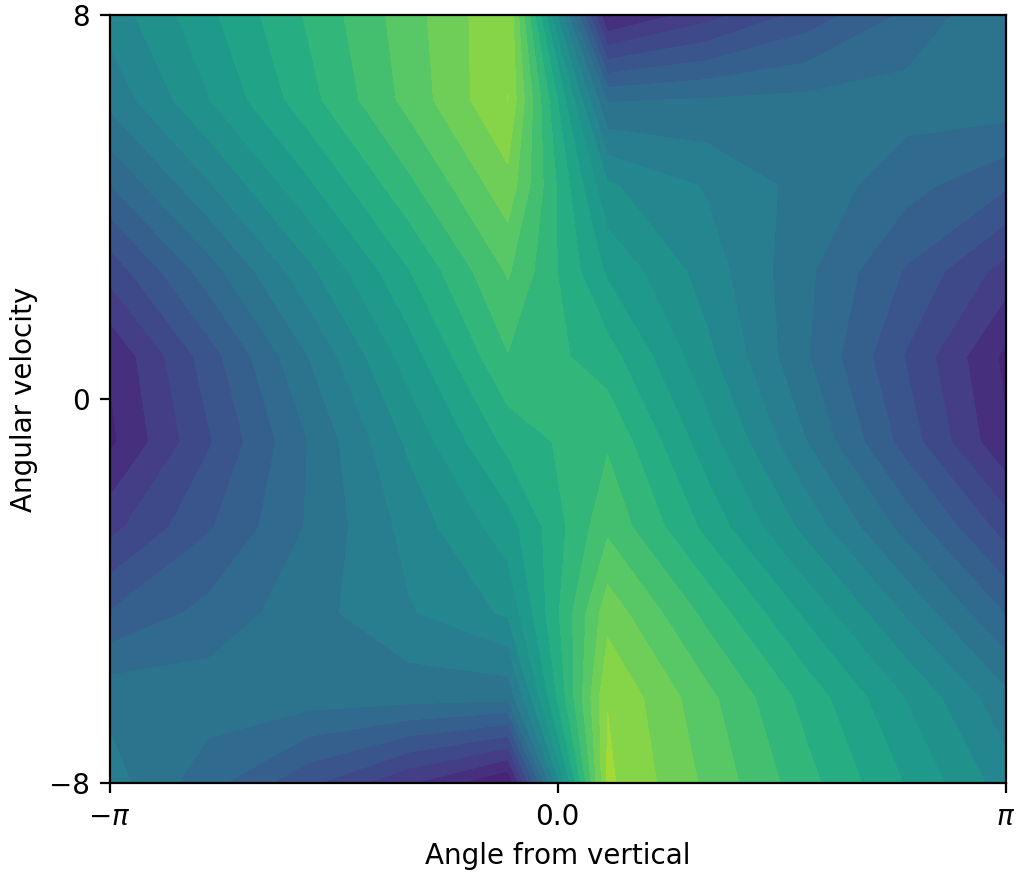
\includegraphics[width=0.9\linewidth,trim=0 0 0 0,clip]{assets/ref_plots/value_model_refcolexps_r10c2_1_ep0}
      \caption{0 episodes}
    \end{subfigure}
    \begin{subfigure}{0.30\linewidth}
      \centering
      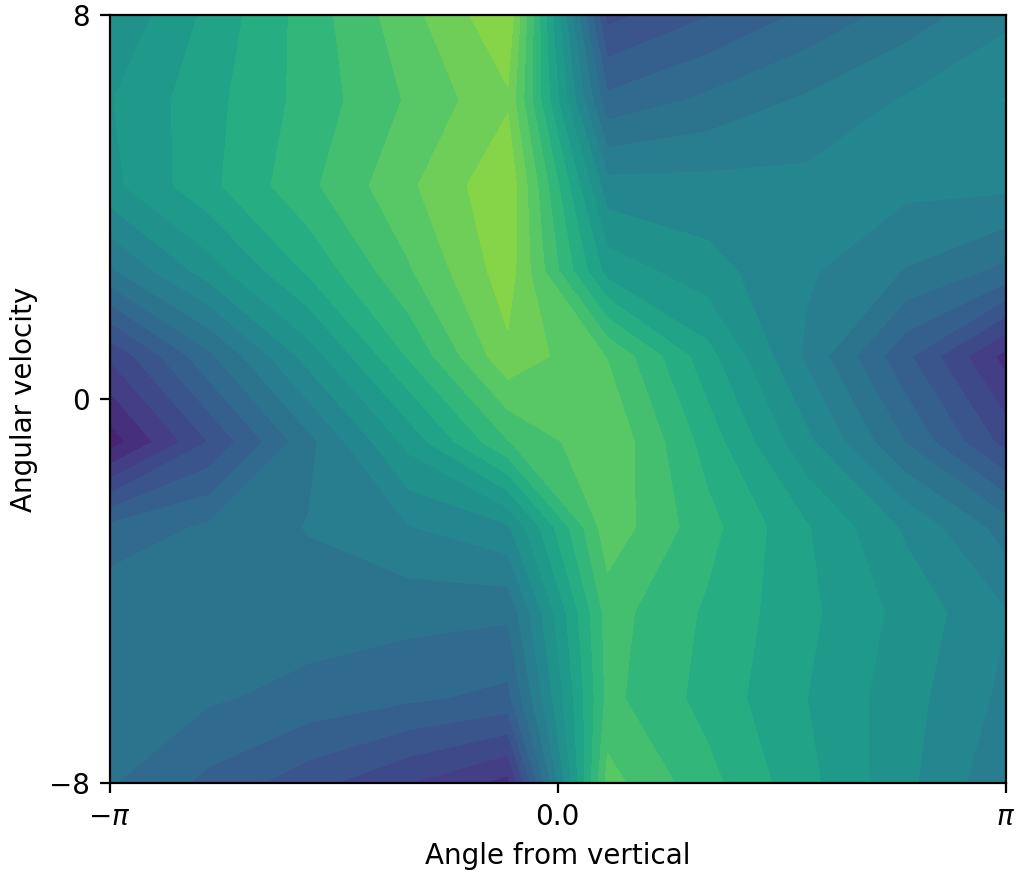
\includegraphics[width=0.9\linewidth,trim=0 0 0 0,clip]{assets/ref_plots/value_model_refcolexps_r10c2_1_ep1000}
      \caption{1000 episodes}
    \end{subfigure}
    \begin{subfigure}{0.30\linewidth}
      \centering
      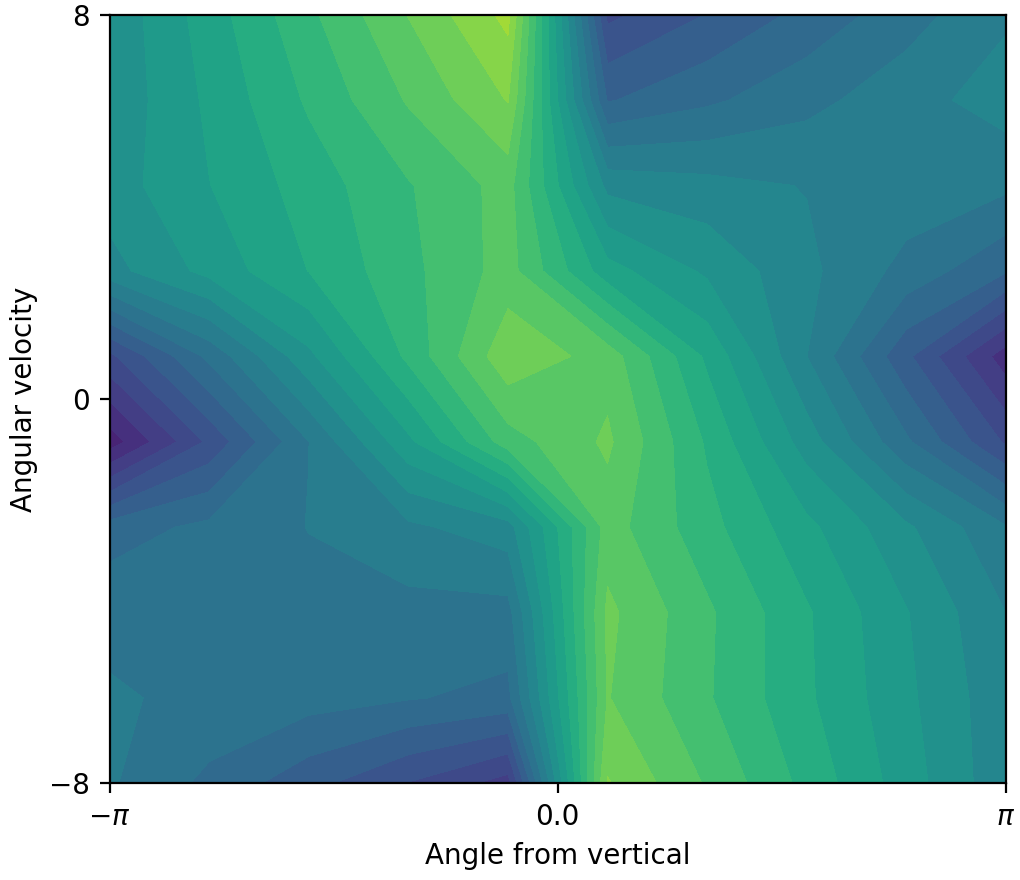
\includegraphics[width=0.9\linewidth,trim=0 0 0 0,clip]{assets/ref_plots/value_model_refcolexps_r10c2_1_ep9900}
      \caption{9900 episodes}
    \end{subfigure}
    \begin{subfigure}{0.05\linewidth}
      \vspace{-2em}
      \centering
      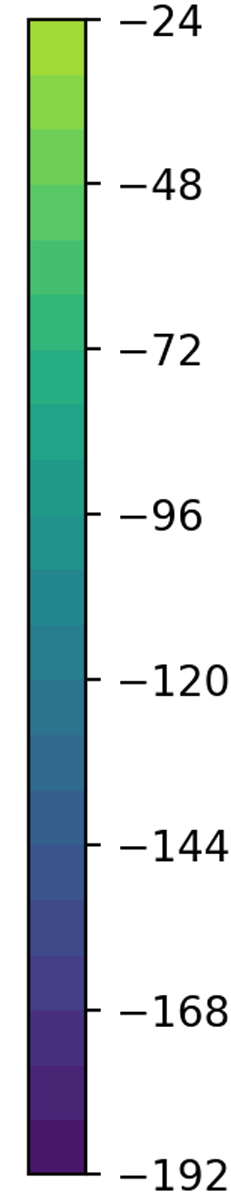
\includegraphics[width=\linewidth,trim=0 0 0 0,clip]{assets/ref_plots/r10c2_colorbar}
    \end{subfigure}
    \caption{Value functions computed by PARL over the course of training. Top Row: 10 rows/10 columns of reference points. Bottom Row: 10 rows/2 columns of reference points. }
  \end{figure}
\end{frame}

\begin{frame}{Interpretability Experiments: Controllers}
  \begin{figure}[t]
    \centering
    \begin{subfigure}{0.30\linewidth}
      \centering
      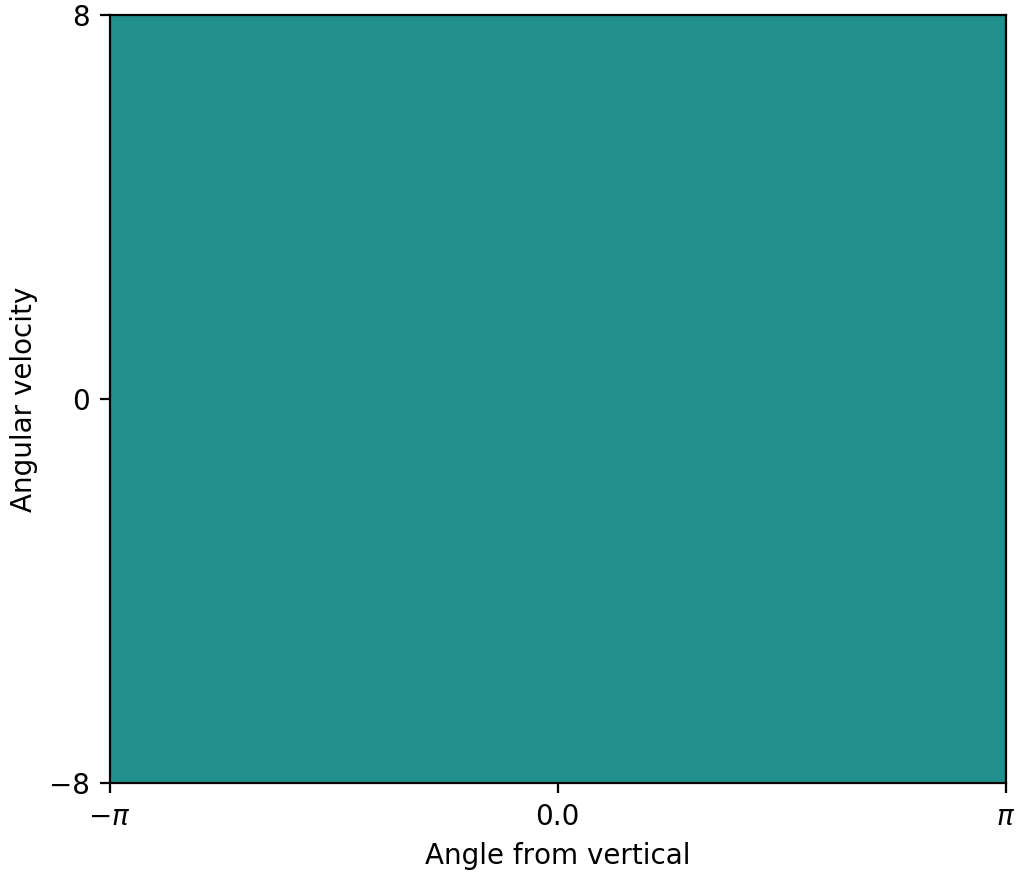
\includegraphics[width=0.9\linewidth,trim=0 0 0 0,clip]{assets/ref_plots/controller_refcolexps_r10c10_1_ep0}
      \caption{0 episodes}
    \end{subfigure}
    \begin{subfigure}{0.30\linewidth}
      \centering
      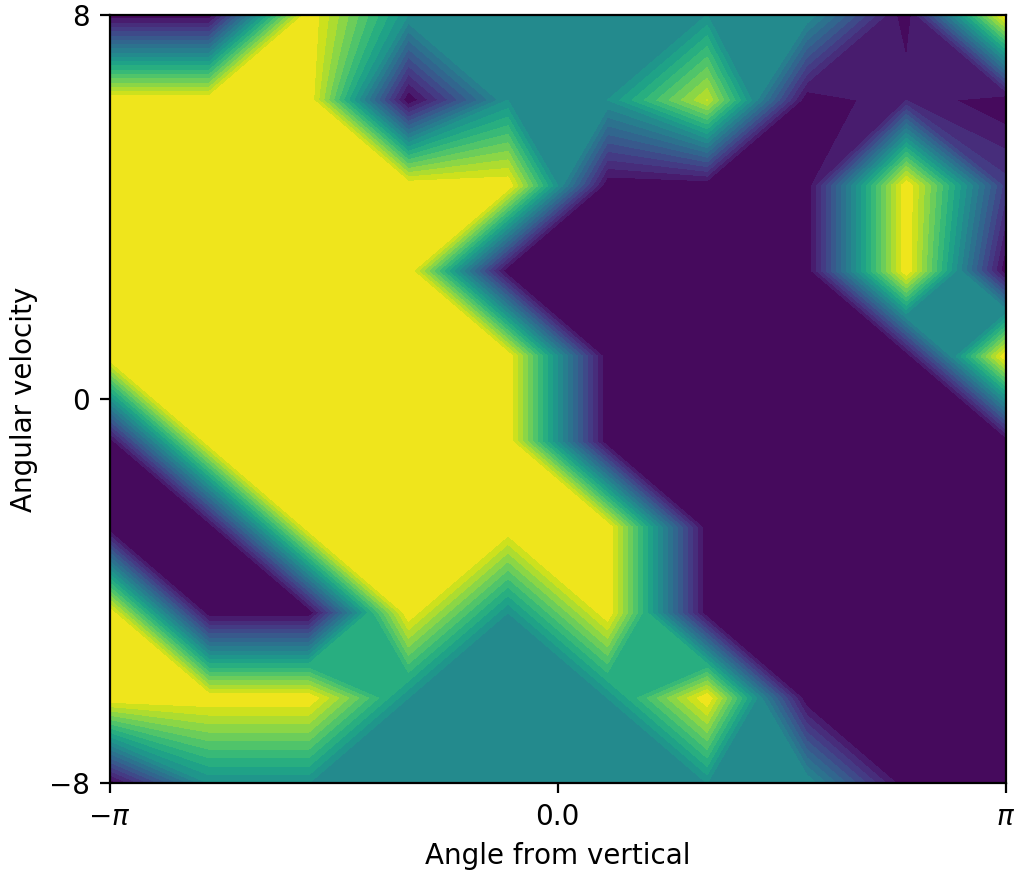
\includegraphics[width=0.9\linewidth,trim=0 0 0 0,clip]{assets/ref_plots/controller_refcolexps_r10c10_1_ep1000}
      \caption{1000 episodes}
    \end{subfigure}
    \begin{subfigure}{0.30\linewidth}
      \centering
      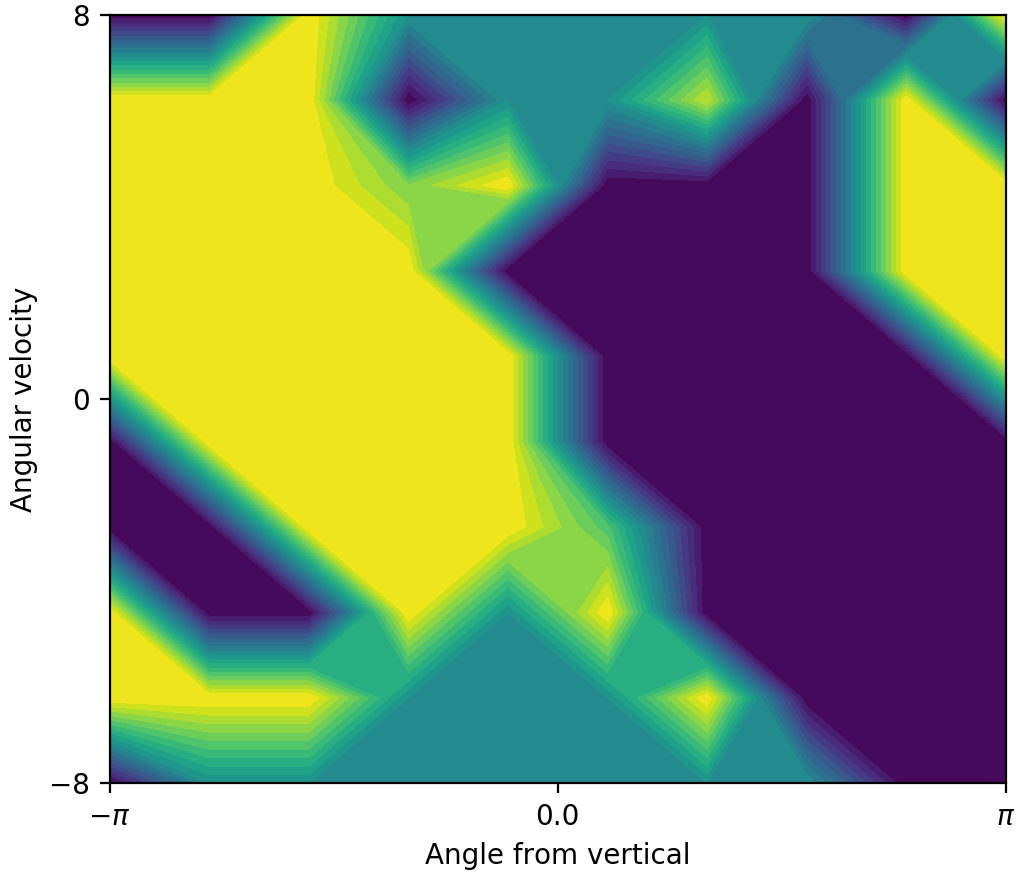
\includegraphics[width=0.9\linewidth,trim=0 0 0 0,clip]{assets/ref_plots/controller_refcolexps_r10c10_1_ep9900}
      \caption{9900 episodes}
    \end{subfigure}
    \begin{subfigure}{0.05\linewidth}
      \vspace{-2em}
      \centering
      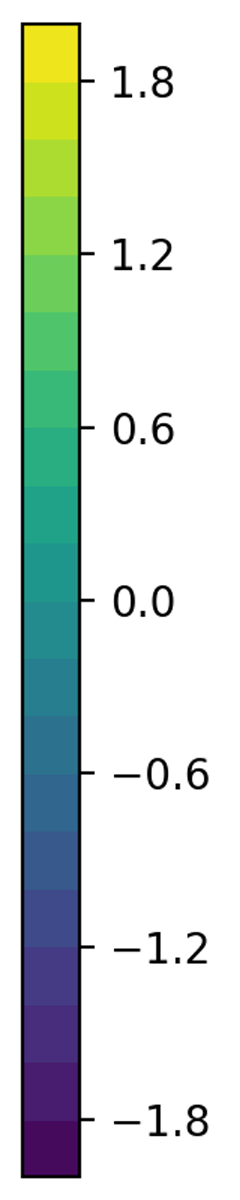
\includegraphics[width=\linewidth,trim=0 0 0 0,clip]{assets/ref_plots/controller_colorbar}
    \end{subfigure}
    \begin{subfigure}{0.30\linewidth}
      \centering
      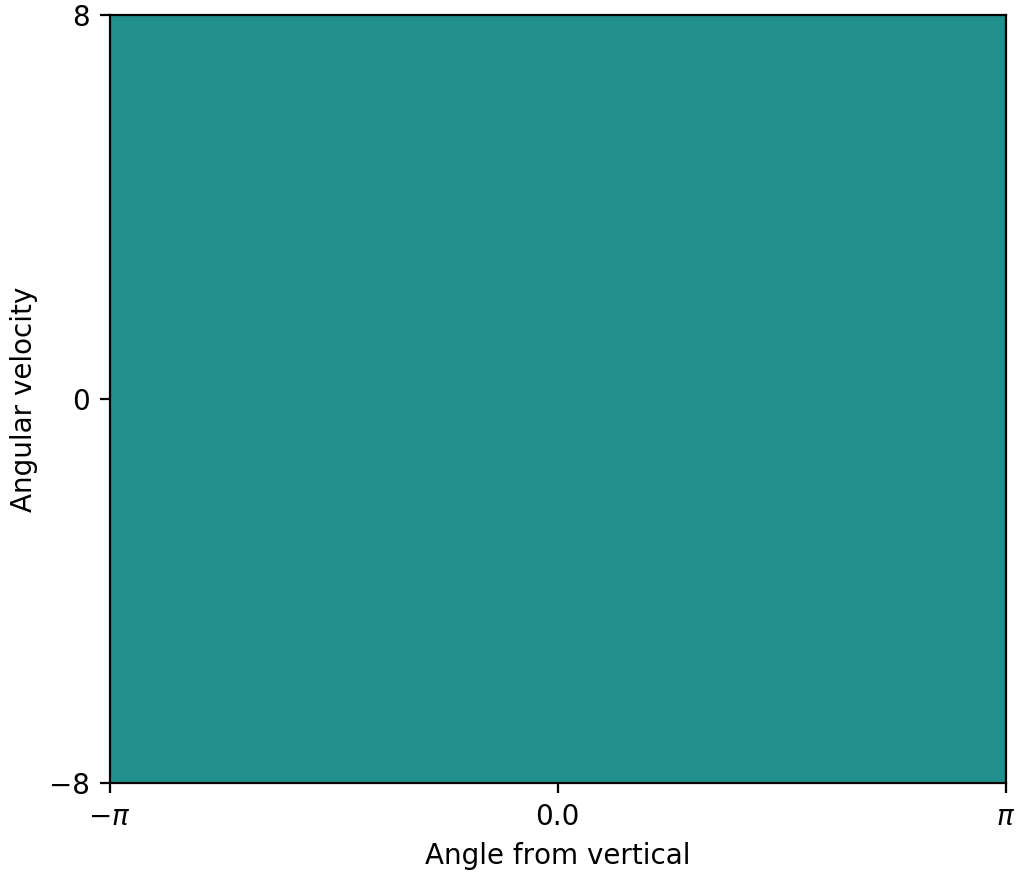
\includegraphics[width=0.9\linewidth,trim=0 0 0 0,clip]{assets/ref_plots/controller_refcolexps_r10c2_1_ep0}
      \caption{0 episodes}
    \end{subfigure}
    \begin{subfigure}{0.30\linewidth}
      \centering
      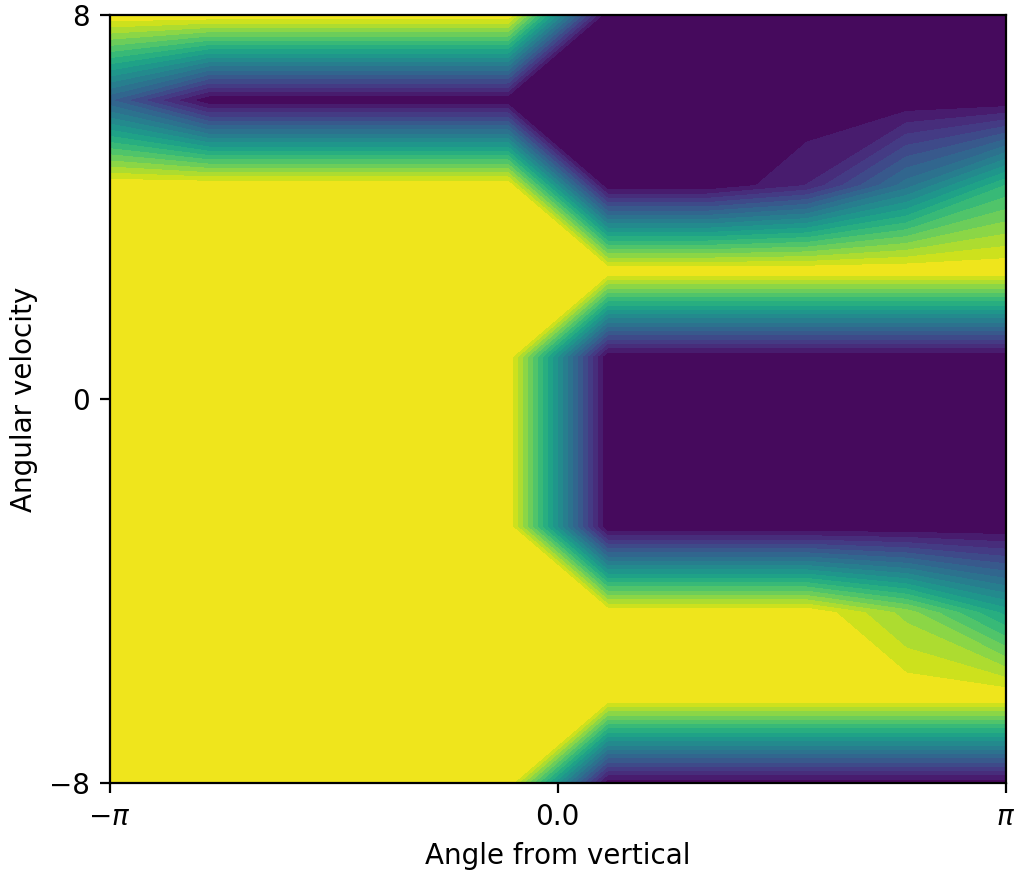
\includegraphics[width=0.9\linewidth,trim=0 0 0 0,clip]{assets/ref_plots/controller_refcolexps_r10c2_1_ep1000}
      \caption{1000 episodes}
    \end{subfigure}
    \begin{subfigure}{0.30\linewidth}
      \centering
      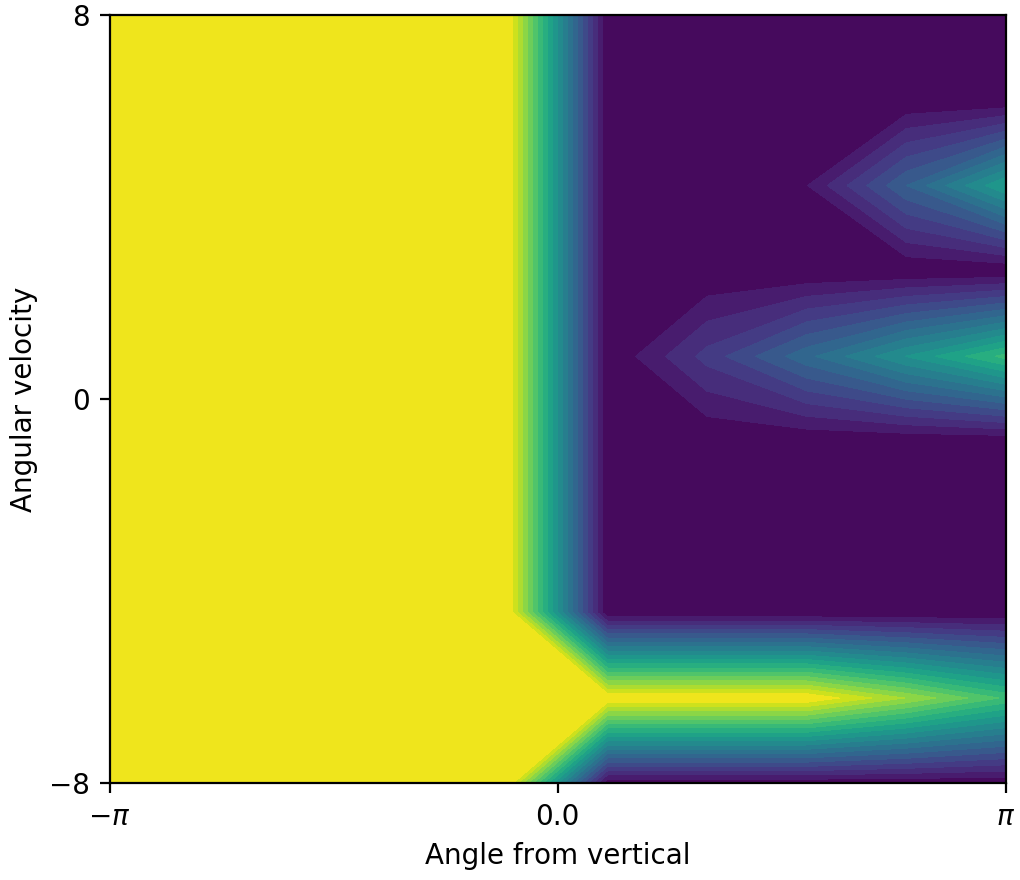
\includegraphics[width=0.9\linewidth,trim=0 0 0 0,clip]{assets/ref_plots/controller_refcolexps_r10c2_1_ep9900}
      \caption{9900 episodes}
    \end{subfigure}
    \begin{subfigure}{0.05\linewidth}
      \vspace{-2em}
      \centering
      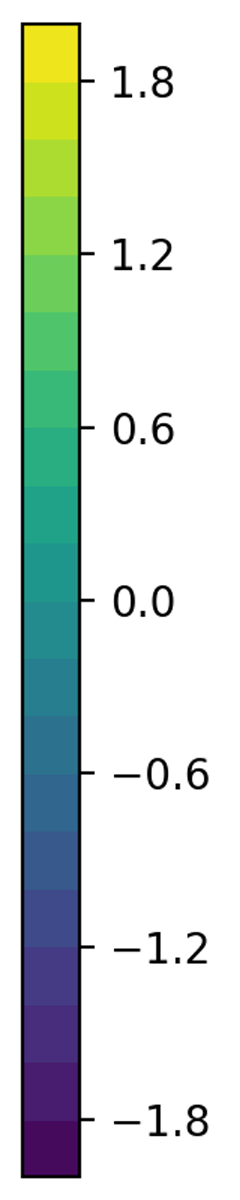
\includegraphics[width=\linewidth,trim=0 0 0 0,clip]{assets/ref_plots/controller_colorbar}
    \end{subfigure}
    \caption{Controllers learned by PARL over the course of training. Top Row: 10 rows/10 columns of reference points. Bottom Row: 10 rows/2 columns of reference points.}
  \end{figure}
\end{frame}


\section{Stability of PARL Controllers}

\begin{frame}{Stability in Control}
  Given a state $\bar{x}$ that we want a system to stay near, how do we design
  controllers which drive the state of the system to $\bar{x}$, even in the
  presence of disturbances?

  Using PARL, we can approximately solve this problem by using the reward function
  \begin{equation*}
    R(x, u) = ||x - \bar{x}||
  \end{equation*}
\end{frame}

\begin{frame}{Lyapunov Functions}
  In discrete time, a \emph{Lyapunov function}\footfullcite{khalil2002nonlinear} $V: X \rightarrow \mathbb{R}$ is a function such that
  \begin{align}
    V(x) \geq 0 \text{ } \forall x \in X \\
    V(\bar{x}) = 0  \\
    V(x_{t+1}) - V(x_t) \leq 0
  \end{align}

  We can find piecewise-affine Lyapunov functions by repeatedly solving a
  linear program~\footfullcite{Rubagotti2012StabilityAO} and refining the PARL
  partition.
\end{frame}

\begin{frame}{Mesh Refinement}
  \begin{algorithm}[H]
      \DontPrintSemicolon
      \KwInput{PWA controller system, maximum number of iterations}
      \KwOutput{Estimate of the region of attraction $P$ and Lyapunov certificate of ES($P$)}
      
      \For{$i < $ maximum iterations}{
          \If{$i > 1$}{
              $\mathcal{X}_i = \mathcal{X}_{ij}, \Omega_{ip}$ \\
              $\mathcal{X} = \bigcup \mathcal{X}_i$
          }    
          Compute the sets $\mathcal{X}_{ij}$ and $\Omega_{ip}$ \\
          Attempt to solve the LP \\
          \If{the LP has a solution}{
              Estimate the region of attraction $P$ \\
              \textbf{Return} the LP solution and $P$
          }
      }
      
      \textbf{Return} $P$ undefined

      \caption{Stability Analysis}
      \label{alg:stability_lp}
  \end{algorithm}
\end{frame}

\begin{frame}{Inverted Pendulum Results}
  \begin{figure}[t]
      \centering
      
      \begin{subfigure}{0.9\linewidth}
          \centering
          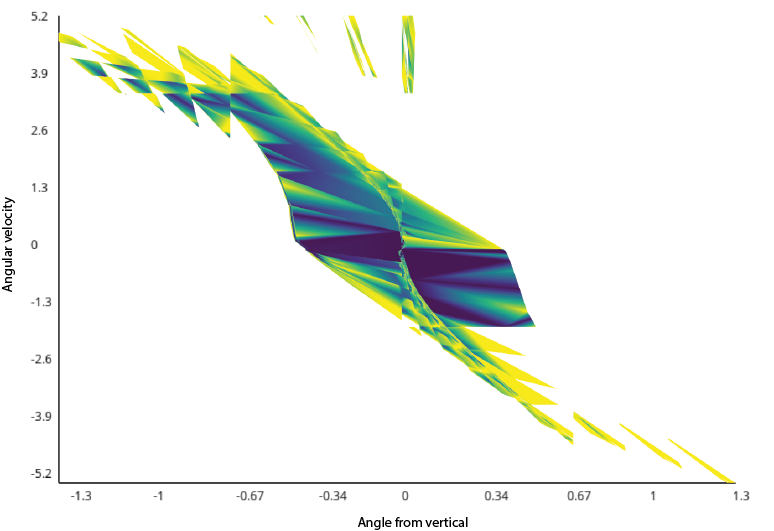
\includegraphics[width=0.95\linewidth,trim=0 0 0 0,clip]{assets/lyapunov}
      \end{subfigure}
      \begin{subfigure}{0.08\linewidth}
          \centering
          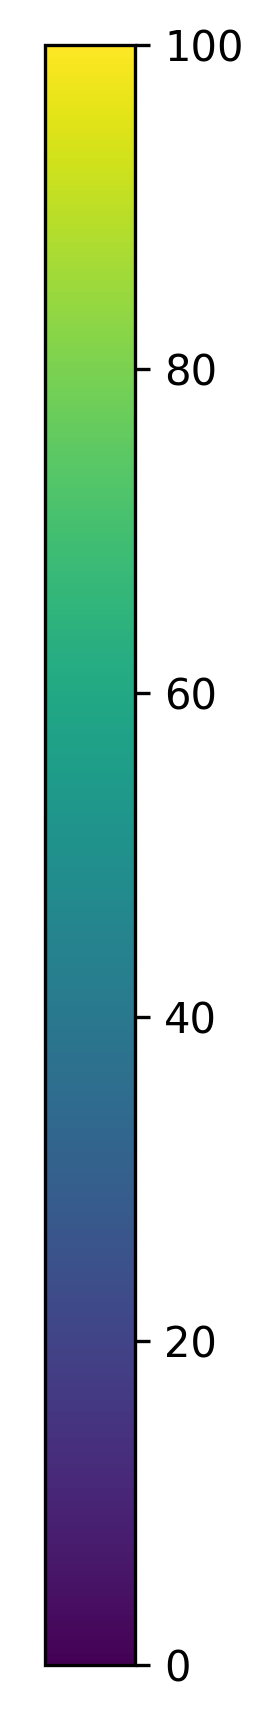
\includegraphics[width=\linewidth,trim=0 0 0 0,clip]{assets/viridis_lyap.png}
      \end{subfigure}
  \end{figure}
\end{frame}

\section{PARL in Reality}

\begin{frame}{Sim2Real}
  Simulation is all well and good, but how does control learning fit into a
  full robotics stack?
\end{frame}

\subsection{PARL+Planning}

\begin{frame}{Nominal Models}
  In most robotics applications, we have access to some kind of nominal model.
  It's not reasonable to throw that model away when we want to do learning.
\end{frame}

\begin{frame}{RL for Tracking Control}
  In order to do RL around a given trajectory, we need to modify the following
  aspects of our MDP formulation:
  \begin{itemize}
    \item The state-space $X$ becomes the $\tilde{x}$ relative to a reference trajectory.
    \item The control space $U$ becomes the $\tilde{u}$ relative to a reference trajectory.
    \item The transition function $P$ changes to incorporate both the movement
      of the frame from $\bar{x}(t)$ to $\bar{x}(t+1)$ and the actual system
      dynamics.
    \item The reward function $R$ must be changed to incorporate some notion of
      instantaneous trajectory-tracking.
  \end{itemize}

\end{frame}

\begin{frame}{PARL Around Trajectory}
  \begin{figure}
    \centering
    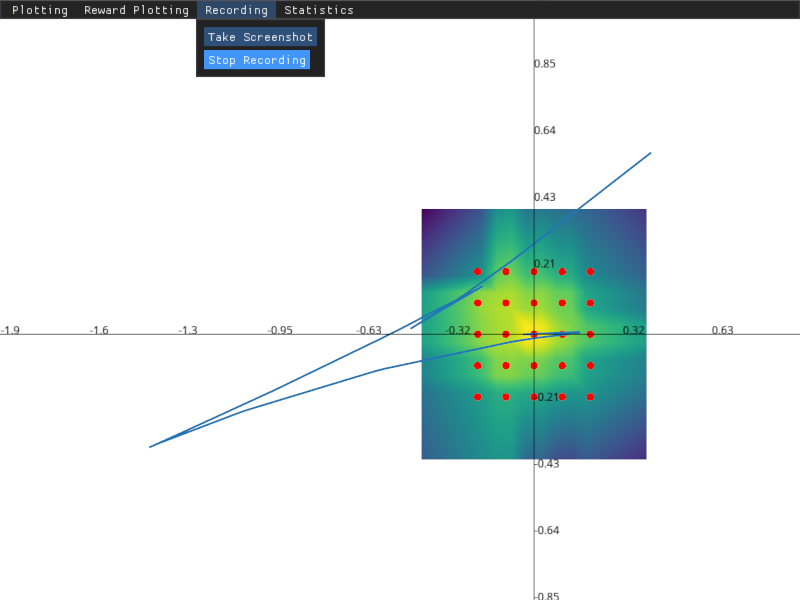
\includegraphics[width=0.8\linewidth]{assets/traj_vals_thumb.png}
  \end{figure}
\end{frame}

\begin{frame}{Open Questions}
  \begin{itemize}
      \item How should reference points be chosen around a trajectory?
      \item How should learning be evaluated?
      \item How should learned information be passed ``upward''?
  \end{itemize}
\end{frame}

\subsection{Safety During Learning}

\begin{frame}{Two Approaches}
  Even with a reference trajectory to help us avoid obstacles, safety needs to
  be addressed for real-robot learning.
  
  In existing literature, there are two main approaches:
  \begin{enumerate}
      \item Incorporate safety into learning objective function.~\footfullcite{7039601}
      \item Rely on a ``backup controller'' to rescue the system if it gets
        close to an unsafe region.~\footfullcite{Berkenkamp2017SafeMR}
  \end{enumerate}
\end{frame}


\section{Questions?}

\section*{Backup}

\begin{frame}{Policy Iteration}
  \begin{algorithm}[H]
      \DontPrintSemicolon
      \KwInput{An MDP $(X, U, R, P)$}
      \KwOutput{A policy $\pi$ optimizing rewards in the MDP}

      Initialize policy $\pi$ and $V_\pi$ \\
      \While {$\pi$ not stationary} {
        Estimate $V_\pi$ (\textbf{Policy Evaluation}) \\
        Set $\pi(x_t) = \argmax_{u_t} \left[r_t +  \gamma V_\pi(x_{t+1})\right]\ \forall x_t \in X$ \\ 
      }

      \textbf{Return} $\pi$

      \caption{Policy Iteration}
      \label{alg:stability_policy_iteration}
  \end{algorithm}
\end{frame}

\begin{frame}{Recursive Least Squares}
  The RLS filter is defined by
  \begin{align*}
    \phi_T &= \left[\begin{array}{l}x_t \\ u_t \end{array}\right] \\
    y_T &= x_{t+1}\\
    P_T &= P_{T-1} - \frac{P_{T-1}\phi_T \phi_T^\top P_{T-1}}{1 + \phi_T^\top P_{T-1} \phi_T} &\text{\emph{(Inverse sample covariance)}} \\
    \theta_T &= \theta_{T-1} + P_T \phi_T \left[y_T - \phi_T^\top \theta_{T-1} \right] &\text{\emph{(RLS parameter estimate)}}
  \end{align*}

  Note $\theta_T = \begin{bmatrix}\hat{A} \\ \hat{B}\end{bmatrix}$, and $\hat{c}$ can be estimated in a similar way.\footnote{See \url{http://cannontwo.com/assets/rls_notes.pdf}}
\end{frame}

\begin{frame}{Least Squares Temporal Difference Learning}

  The LSTD filter is a modified RLS filter, defined by:
  \begin{align*}
    \Delta &= \phi_T(x_t) - \gamma \phi_T(x_{t+1})\\
    C_{t+1} &= C_T - \frac{C_T \phi_T(x_t) \Delta^\top C_T}{1 + \Delta^\top C_t \phi_T(x_t)}\\
    d_{t+1} &= d_T + \phi_T(x_t)r_t
  \end{align*}
  and the corresponding parameters are given by $C_T d_T$, from which $V_0$ and $V_x$ can be extracted for each partition region.
\end{frame}

\begin{frame}{Kinds of Stability}
  In addition to basic Lyapunov stability, we have
  \begin{itemize}
    \item \emph{Asymptotic stability}: $V(x_{t+1}) - V(x) < 0$, and so the system monotonically proceeds to $\bar{x}$.
    \item \emph{Exponential stability}: If $V(x)$ decreases faster than an exponential function of $x$, and so the system proceeds ``quickly'' to $\bar{x}$.
  \end{itemize}
  For this stability exploration, we only consider basic Lyapunov stability.
\end{frame}

\begin{frame}{Learning Errors}
  Suppose that the real system is of the form
  \begin{equation*}
    x_{t+1} = f(x_t, u_t) = F(x_t) + G(x_t)u_t
  \end{equation*}
  and we are given a nominal model of the form 
  \begin{equation*}
    \bar{x}_{t+1} = \bar{F}(x_t) + \bar{G}(x_t)u_t
  \end{equation*}
  Then we want to estimate $\hat{F}, \hat{G}$ such that 
  \begin{align*}
    x_{t+1} &\approx \bar{x}_{t+1} + \hat{F}(x_t) + \hat{G}(x_t)u_t \\
    &\approx \left(\bar{F} + \hat{F}\right)(x_t) + \left(\bar{G} + \hat{G}\right)(x_t)u_t
  \end{align*}
\end{frame}

\begin{frame}{Tracking Control Formulation}
  Given a nominal trajectory of the form $\bar{x}(t), \bar{u}(t)$, we can set
  up a tracking control problem by transforming our state-space:
  \begin{align*}
    \tilde{x}_t &= x_t - \bar{x}(t) \\
    \tilde{u}_t &= u_t - \bar{u}(t)
  \end{align*}
  This gives us an analogous linearization to the stabilization problem:
  \begin{align*}
    \tilde{x}_{t+1} &= f(x_t, u_t) - f(\bar{x}(t), \bar{u}(t)) \\
                    &\approx A(t)\tilde{x}_t + B(t)\tilde{u}_t
  \end{align*}
  This time-varying linear approximation can be learned by PARL, assuming that
  the PARL reference points move along with the trajectory-local frame.
\end{frame}

\begin{frame}{Safety via Optimization}
  \begin{columns}
    \begin{column}{0.5\textwidth}
    \begin{figure}
      \centering
      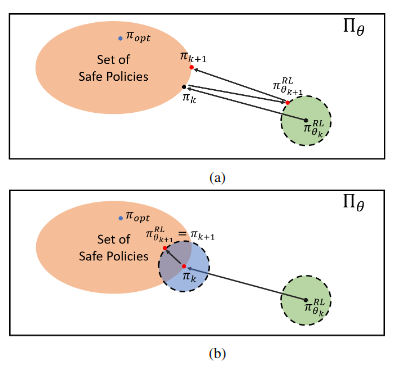
\includegraphics[width=\linewidth]{assets/policy_projection.png}
    \end{figure}
  \end{column}

  \begin{column}{0.5\textwidth}
    \begin{itemize}
      \item Safety as an additional term in reward function
      \item Safety as a constraint on allowed actions, resolved via optimization 
    \end{itemize}
  \end{column}\footfullcite{7039601}
  \end{columns}

\end{frame}

\begin{frame}{Safety via Backup Controller}
  \begin{figure}
    \centering
    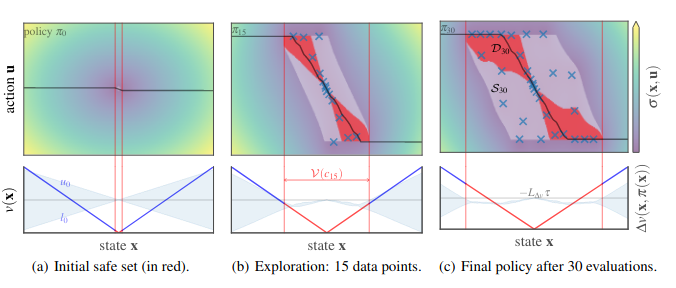
\includegraphics[width=0.9\linewidth]{assets/safety_region.png}
  \end{figure}
  Using an initial controller, the learning process safe
  throughout. \footfullcite{Berkenkamp2017SafeMR}

  But where does this controller come from? What are we learning?
\end{frame}

\end{document}
